\documentclass{article}
\usepackage[utf8]{inputenc}
\usepackage[margin=1in]{geometry}

\title{452 - Homework 5}
\author{Victor Zhang}
\date{February 26, 2021}

\usepackage[utf8]{inputenc}
\usepackage{amsmath}
\usepackage{amsfonts}
\usepackage{natbib}
\usepackage{graphicx}
% \usepackage{changepage}
\usepackage{amssymb}
\usepackage{xfrac}
% \usepackage{bm}
% \usepackage{empheq}
\usepackage{tikz}
\usetikzlibrary{arrows,automata}
\usepackage{dirtytalk}

\newcommand{\contra}{\raisebox{\depth}{\#}}

\newenvironment{myindentpar}[1]
  {\begin{list}{}
          {\setlength{\leftmargin}{#1}}
          \item[]
  }
  {\end{list}}

\pagestyle{empty}

\begin{document}

\maketitle
% \begin{center}
% {\huge Econ 482 \hspace{0.5cm} HW 3}\
% {\Large \textbf{Victor Zhang}}\
% {\Large February 18, 2020}
% \end{center}

\section*{2.11}
We follow exactly the procedure given in the proof of 2.20 to get
% \begin{tikzpicture}[->,>=stealth',shorten >=1pt,auto,node distance=3.7cm,
%         scale = 1,transform shape]

%   \node[state,initial] (0) {$0$};
%   \node[state] (1) [right of=0] {$1$};
%   \node[state] (2) [right of=1] {$2$};
%   \node[state] (3) [below left of=2] {$3$};
%   \node[state] (4) [below left of=3] {$4$};
%   \node[state] (5) [below right of=2] {$5$};
%   \node[state] (6) [below right of=5] {$6$};
%   \node[state] (7) [right of=2] {$7$};
%   \node[state] (8) [right of=7] {$8$};
%   \node[state,accepting] (end) [above of=2] {$end$};

%   \path (0) edge              node {$\epsilon,\epsilon\to\$$} (1)
%         (1) edge [bend right=4]             node [below] {$\epsilon,\epsilon\to E$} (2)
%         (2) edge [bend left=15]  node {$\epsilon,E\to T$} (3)
%         (3) edge [bend right=5] node {$\epsilon,\epsilon \to \epsilon$} (2)
%         (3) edge              node {$\epsilon,\epsilon \to +$} (4)
%         (4) edge [bend left] node {$\epsilon,\epsilon \to E$} (2)
%         (2) edge [bend left=10]             node {$\epsilon,T \to F$} (5)
%         (5) edge              node [right] {$\epsilon,\epsilon \to \epsilon$} (2)
%         (5) edge              node {$\epsilon,\epsilon \to \times$} (6)
%         (6) edge [bend left=13] node {$\epsilon,\epsilon \to T$} (2)
%         (2) edge [loop left]  node [above=4] {$s,s \to \epsilon \;\forall s \in \Sigma$} (2)
%         (2) edge [loop right] node [below right]{$\epsilon,F \to a$} (2)
%         (2) edge [bend left=5] node {$\epsilon,F \to )$} (7)
%         (7) edge              node {$\epsilon,\epsilon \to E$} (8)
%         (8) edge [bend right] node {$\epsilon,\epsilon \to ($} (2)
%         (2) edge              node {$\epsilon,\$ \to \epsilon$} (end);

% \end{tikzpicture}

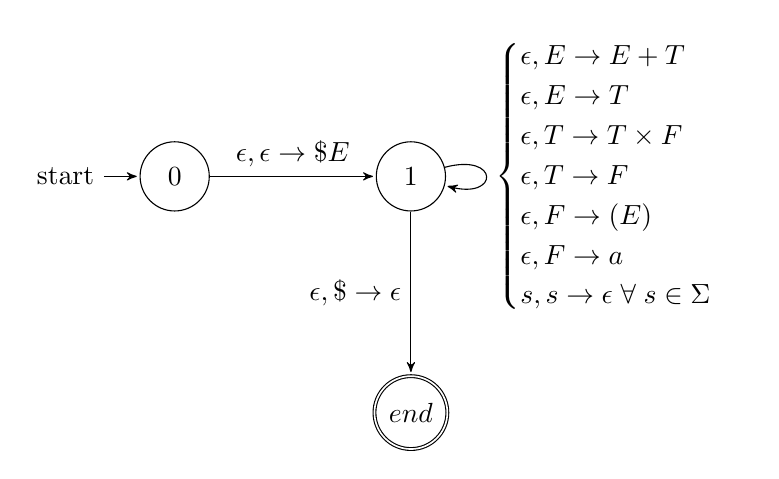
\begin{tikzpicture}[->,>=stealth',shorten >=1pt,auto,node distance=3cm,
        scale = 1,transform shape]

  \node[state,initial] (0) {$0$};
  \node[state] (1) [right of=0] {$1$};
  \node[state,accepting] (end) [below of=1] {$end$};

  \path (0) edge              node {$\epsilon,\epsilon\to\$ E$} (1)
        (1) edge              node [left] {$\epsilon,\$\to\epsilon$} (end)
        (1) edge [loop right] node [align=left]{$
          \begin{cases}
            \epsilon,E \to E + T\\
            \epsilon,E \to T\\
            \epsilon,T \to T \times F\\
            \epsilon,T \to F\\
            \epsilon,F \to (E)\\
            \epsilon,F \to a\\
            s,s \to \epsilon \;\forall\; s \in \Sigma
          \end{cases}$} (1);

\end{tikzpicture}

\section*{2.25}
Let $M$ be a PDA accepting $A$ generated as by theorem 2.20. Duplicate $M$ and call it $M'$. Make an empty transition $\epsilon,\epsilon\to\epsilon$ from the \say{main} state of $M$ to the \say{main} state of $M'$. (The main state is the state generated right at the end of step 1 in the proof of 2.20. In the solution to the previous homework problem, the main state is labelled 1.) In $M$, replace all transitions $\{s,s \to \epsilon \;:\; s \text{ terminal}\}$ with $\epsilon,s \to \epsilon$. Fix the start state of the combined machine to be the start state of $M$.\\
This new machine accepts any suffix of $A$, since we may nondeterministically \say{ignore} any (potentially empty) prefix of a derivation in $A$ by cycling in $M$ and read the suffix by transitioning to $M'$ and cycling in $M'$ $\Box$

\section*{2.30.a}
Let $p$ be arbitrary and put $s = 0^p1^p0^p1^p = uvxyz$ as dictated by the pumping lemma. For simplicity, denote by a \say{piece} of $s$ one of the 4 runs of $x^p$. Both $v$ and $y$ must contain only one symbol, since otherwise $uvvxyyz$ is clearly not in the language. One case is that $vxy$ is totally contained in one piece. WLOG suppose it is contained in the first piece. But then $uxz = 0^{p-j}1^p0^p1^p$ for some $j > 0$, so is not in the language. We may argue similarly for all other similar cases. The other case is that $v = x^a$, $y = (\neg x)^b$, $x \in \Sigma$. Note $vxy$ may only span two pieces, so $uxz$ will necessarily have two pieces that are longer than the other two, so is not in the language. Then by pumping lemma, this is not a CFL $\Box$

\section*{2.30.d}
Let $p$ be arbitrary and put $s = t_1\#t_2 = a^pb^p\#a^pb^p = uvxyz$. Note neither of $v$ or $y$ may contain symbol $\#$, since otherwise $uxz$ would have $k = 1$. If $vxy$ is wholly contained in either $t_1$ or $t_2$, clearly $uxz$ will not be in the language. The other case is that $vxy$ spans $t_1$ and $t_2$, in which case $v = b^j$, $y = a^l$ and clearly $uxz$ is not in the language. Then by pumping lemma, the language is not a CFL $\Box$

\section*{2.32}
Let $p$ be arbitrary and put $s = 1^p3^p2^p4^p = uvxyz$. We notice this is similar to the string we used in 2.30.a. Further, we recall that all nontrivial pumping lemma cases in that problem failed because one \say{piece} had a different length than the other piece with the same symbol. Thus, all cases will fail similarly for $s$ and by pumping lemma, the language is not context free $\Box$

\section*{2.48.a}
We note the shortest string in the language is $a1a$, $a \in \Sigma$. An equivalent statement of the necessary condition is $\{x1z \;:\; x \in \Sigma^*, z \in \Sigma^*, |x| \leq 2|z|-1, |z| \leq 2|x|-1\}$. This language is generated by the following context-free grammar
\begin{equation*}
\begin{cases}
S \to ABSBA \;|\; A1A\\
A \to 0 \;|\; 1\\
B \to 0 \;|\; 1 \;|\; \epsilon
\end{cases}
\end{equation*}

\section*{2.48.b}
Let $p$ be arbitrary and put $s = 0^{p+2}10^p10^{p+2} = uvxyz$. By \say{third} we mean one of the three contiguous thirds of the string in question. If we pick $vxy$ to be wholly contained in the first or third third, $uvvxyyz$ is clearly not in the language, since then either the first or last third of the new string contains one of the only two 1s in the string. In fact, if neither of $v$ or $y$ contain a 1, the new string $uvvxyyz$ fails for the same reason. Finally WLOG suppose $v$ contains a 1. Then $y$ cannot contain a 1. If $y$ is wholly contained in the second third, $uvvxyyz$ fails because the last third absorbs the second 1. If $y$ is wholly contained in the last third, $uvvxyyz$ fails because the first third absorbs the first 1. Thus, by pumping lemma, the language is not regular $\Box$

\section*{2.24}
We split the language $E$ into 3 disjoint languages: $A$ with condition $j < i$, $B$ with condition $i < j < 2i$, and $C$ with condition $j > 2i$. It suffices to show $A,B,C$ are CFLs, since CFLs are closed under union. $A$ is generated by the following grammar
\begin{equation*}
\begin{cases}
S \to aT\\
T \to ATb \;|\; \epsilon\\
A \to aA \;|\; a
\end{cases}
\end{equation*}
$B$ is generated by
\begin{equation*}
\begin{cases}
S \to aaTbbb\\
T \to aTB \;|\; \epsilon\\
B \to b \;|\; bb
\end{cases}
\end{equation*}
and $C$ is generated by
\begin{equation*}
\begin{cases}
S \to TB\\
T \to aTBB \;|\; \epsilon\\
B \to bB \;|\; b
\end{cases}
\end{equation*}
$\Box$

\section*{2.37}
Our proof will be very similar to Sipser's proof of the regular pumping lemma. Suppose grammar $G$ generates $A$. Denote by $v$ the number of variables in $G$. Denote by $b$ the maximum number of symbols to the right of a rule. Put $k = b^{3v+1}$. Let $s$ be a string with length at least $k$ and consider the minimal parse tree for $s$. By pigeonhole, there is some variable $R$ which appears at least 4 times in the longest root to leaf path. In particular, it must appear in the bottom $3v+1$ levels of the path. As in Sipser's proof, we may write $R \overset{*}{\to} v_1v_2v_3xy_3y_2y_1$. By regular pumping lemma, at least one of $v_1v_2v_3$ or $y_3y_2y_1$ is nonempty. If both are nonempty, we are done. Otherwise WLOG suppose that $v_1v_2v_3$ is nonempty. Then $R \overset{*}{\to} v_1v_2v_3m$, $R \overset{*}{\to} v_2v_3m$, $R \overset{*}{\to} v_3m$. By regular pumping lemma, none of $v_1,v_2,v_3$ are empty. Then clearly we may pump $v=v_1$, $y=v_3$. Finally note since the first occurrence of $R$ is the root of a subtree of height at most $3v+1$, $|v_1v_2v_3xy_3y_2y_1| \leqslant k$, so we are done $\Box$

% TODO: 2.30.d after clarification
%       2.11 with simplification of pushing multiple things to stack


\end{document}

% List of tex snippets:
%   - tex-header (this)
%   - R      --> \mathbb{R}
%   - Z      --> \mathbb{Z}
%   - B      --> \mathcal{B}
%   - E      --> \mathcal{E}
%   - M      --> \mathcal{M}
%   - m      --> \mathfrak{m}({#1})
%   - normlp --> \norm{{#1}}_{L^{{#2}}}

